\documentclass[a4paper, 10.5pt]{ctexart}

% !!!重要提示!!! 请使用 XeLaTeX 编译此文件以获得最佳字体和排版效果。

% --- 导包 Preamble ---
\usepackage[left=1.0cm, right=1.0cm, top=1.4cm, bottom=1.4cm]{geometry}
\usepackage{graphicx}
\usepackage{xcolor}
\usepackage{fontspec}
\usepackage{enumitem}
\usepackage[explicit]{titlesec}
\usepackage{microtype}
\usepackage{fontawesome5}
\usepackage{academicons}
\usepackage{hyperref}
\usepackage{etoolbox}
\usepackage{array}
\usepackage{tikz}
\newsavebox{\headerbox}
% 论文条目之间的间距（模板里 \parskip 在两栏中不起作用，改用显式 \vspace）
\newlength{\pubgap}\setlength{\pubgap}{0.45em}
% 节标题前的间距（titlesec 的节前距在两栏里不起作用，改用显式 \vspace*）
\newlength{\secgap}\setlength{\secgap}{0.8em}
% 左栏的整段文字（Interests 简介、Hobbies）：两端对齐并允许连字符断词，
% 免得窄栏里右边缘参差不齐；列表式的短行仍沿用左栏的左对齐、不断词。
\newcommand{\leftpara}[1]{{\rightskip=0pt\relax\parfillskip=0pt plus 1fil\relax\hyphenpenalty=1500\relax\exhyphenpenalty=1500\relax\tolerance=4000\relax\emergencystretch=2em\relax #1\par}}

% --- 颜色定义 Colors ---
\definecolor{PrimaryColor}{HTML}{003366}
\definecolor{DescriptionGray}{HTML}{444444}
\definecolor{VenueColor}{HTML}{B31B1B}

% --- 字体设置 Fonts (XeLaTeX) ---
% 字体源：项目根目录 fonts/（站点统一字体集）。
% 当前文件位于 static/uploads/CV.tex，相对路径为 ../../fonts/。
% 中文：方正新书宋简体
\setCJKmainfont[
  Path = ../../fonts/方正新书宋简体/ ,
  AutoFakeBold = 2.0
]{方正新书宋简体.ttf}

% 英文衬线：CMU Serif
\setmainfont[
  Path = ../../fonts/cmu-serif/ ,
  Extension = .ttf,
  UprightFont = cmunrm,
  BoldFont = cmunbx,
  ItalicFont = cmunti,
  BoldItalicFont = cmunbi
]{CMU Serif}

% 英文无衬线：CMU Sans Serif
\setsansfont[
  Path = ../../fonts/cmu-sans-serif/ ,
  Extension = .ttf,
  UprightFont = cmunss,
  BoldFont = cmunsx,
  ItalicFont = cmunsi,
  BoldItalicFont = cmunso
]{CMU Sans Serif}

% --- 超链接 ---
\hypersetup{
  colorlinks=true,
  linkcolor=PrimaryColor,
  urlcolor=PrimaryColor,
  citecolor=PrimaryColor,
  pdfborder={0 0 0},
}

% --- 全局设置 ---
\pagestyle{empty}
\setlength{\parindent}{0pt}
\setlength{\parskip}{0.4em}
\setlength{\emergencystretch}{3em}
\setlist{itemsep=0.2em, parsep=0pt, topsep=0.3em, leftmargin=1.2em}

% --- Section 标题样式 ---
\titleformat{\section}
  {\normalfont\large\bfseries\color{PrimaryColor}}
  {}
  {0em}
  {#1}
  [\vspace{0.2ex}\hrule height 0.6pt]
\titlespacing*{\section}{0pt}{1.8ex}{1.0ex}

% --- 自定义命令 Custom Commands ---

% 子标题 (subsection)：深蓝粗体小号；与上下 entry 紧贴
\newcommand{\subSection}[1]{%
  \vspace{-0.15em}%
  \noindent{\color{PrimaryColor}\textbf{\small #1}}\par%
  \vspace{-0.1em}%
}

% 经历条目：#1=职位@机构, #2=时间(可空), #3=描述(可空)
% 标题左对齐，时间用 \hfill 右对齐；描述行紧跟标题
\newcommand{\jobEntry}[3]{%
  \noindent\textbf{#1}%
  \notblank{#2}{\hfill{\color{DescriptionGray}\small #2}}{}%
  \notblank{#3}{\par\vspace{0.05em}\noindent{\color{DescriptionGray}\small\textit{#3}}}{}%
  \par\vspace{0.35em}%
}

% 五圆点技能条
\newcommand{\filledDot}{\textcolor{PrimaryColor}{\small\textbullet}}
\newcommand{\emptyDot}{\textcolor{DescriptionGray}{\small$\circ$}}
\newcommand{\skillRow}[2]{%
  % #1 = 技能名, #2 = 等级 1-5
  #1 &
  \ifnum#2>0\filledDot\else\emptyDot\fi\,%
  \ifnum#2>1\filledDot\else\emptyDot\fi\,%
  \ifnum#2>2\filledDot\else\emptyDot\fi\,%
  \ifnum#2>3\filledDot\else\emptyDot\fi\,%
  \ifnum#2>4\filledDot\else\emptyDot\fi%
  \\
}

\begin{document}

% =====================================================================
% Header：照片 tikz overlay 浮于右上角，文字相对整页居中
% =====================================================================
% 把文字部分先 sbox，自动测量真实高度
\sbox{\headerbox}{%
  \begin{minipage}{\dimexpr\textwidth-1cm\relax}
    \centering
    {\fontsize{22pt}{26pt}\selectfont\bfseries\color{PrimaryColor}王司晨 (Sichen Wang)}\\[0.45em]
    {\color{DescriptionGray}
      \raisebox{-0.2em}{
\includegraphics[height=1em]{yourphoto.png}}\ \href{https://sichenwang.com}{sichenwang.com} \quad
      \faIcon{github}\ \href{https://github.com/sichen-wang}{github.com/sichen-wang} \quad
      {\aiOrcid}\ \href{https://orcid.org/0009-0008-3734-4006}{0009-0008-3734-4006}\\[0.2em]
      \faIcon{envelope}\ \href{mailto:sichenwang@cuhk.edu.cn}{sichenwang@cuhk.edu.cn} \quad
      \faIcon{envelope}\ \href{mailto:me@sichenwang.com}{me@sichenwang.com} \quad
      \faIcon{linkedin}\ \href{https://www.linkedin.com/in/sichen-wang/}{sichen-wang}}
  \end{minipage}%
}

% 占位 rule：向 LaTeX 报告 header 高度，确保后续内容从 (top margin + H) 开始
\noindent\rule{0pt}{\dimexpr\ht\headerbox+\dp\headerbox\relax}%

% 用 tikz overlay 在精确坐标放置文字和照片，强制底部对齐
\begin{tikzpicture}[remember picture, overlay]
  % 文字框：顶部 anchor=north，锁定到 page top - 1.4cm（即 body top），相对页面中心向左偏 0.5cm
  \node[anchor=north, inner sep=0pt] at
    ([xshift=-0.5cm, yshift=-1.4cm]current page.north)
    {\usebox{\headerbox}};
  % 照片：底部 anchor=south east，锁定到 page top - (1.4cm + H)，即文字底部
  \node[anchor=south east, inner sep=0pt] at
    ([xshift=-1.7cm, yshift={\dimexpr -1.4cm-\ht\headerbox-\dp\headerbox\relax}]current page.north east)
    {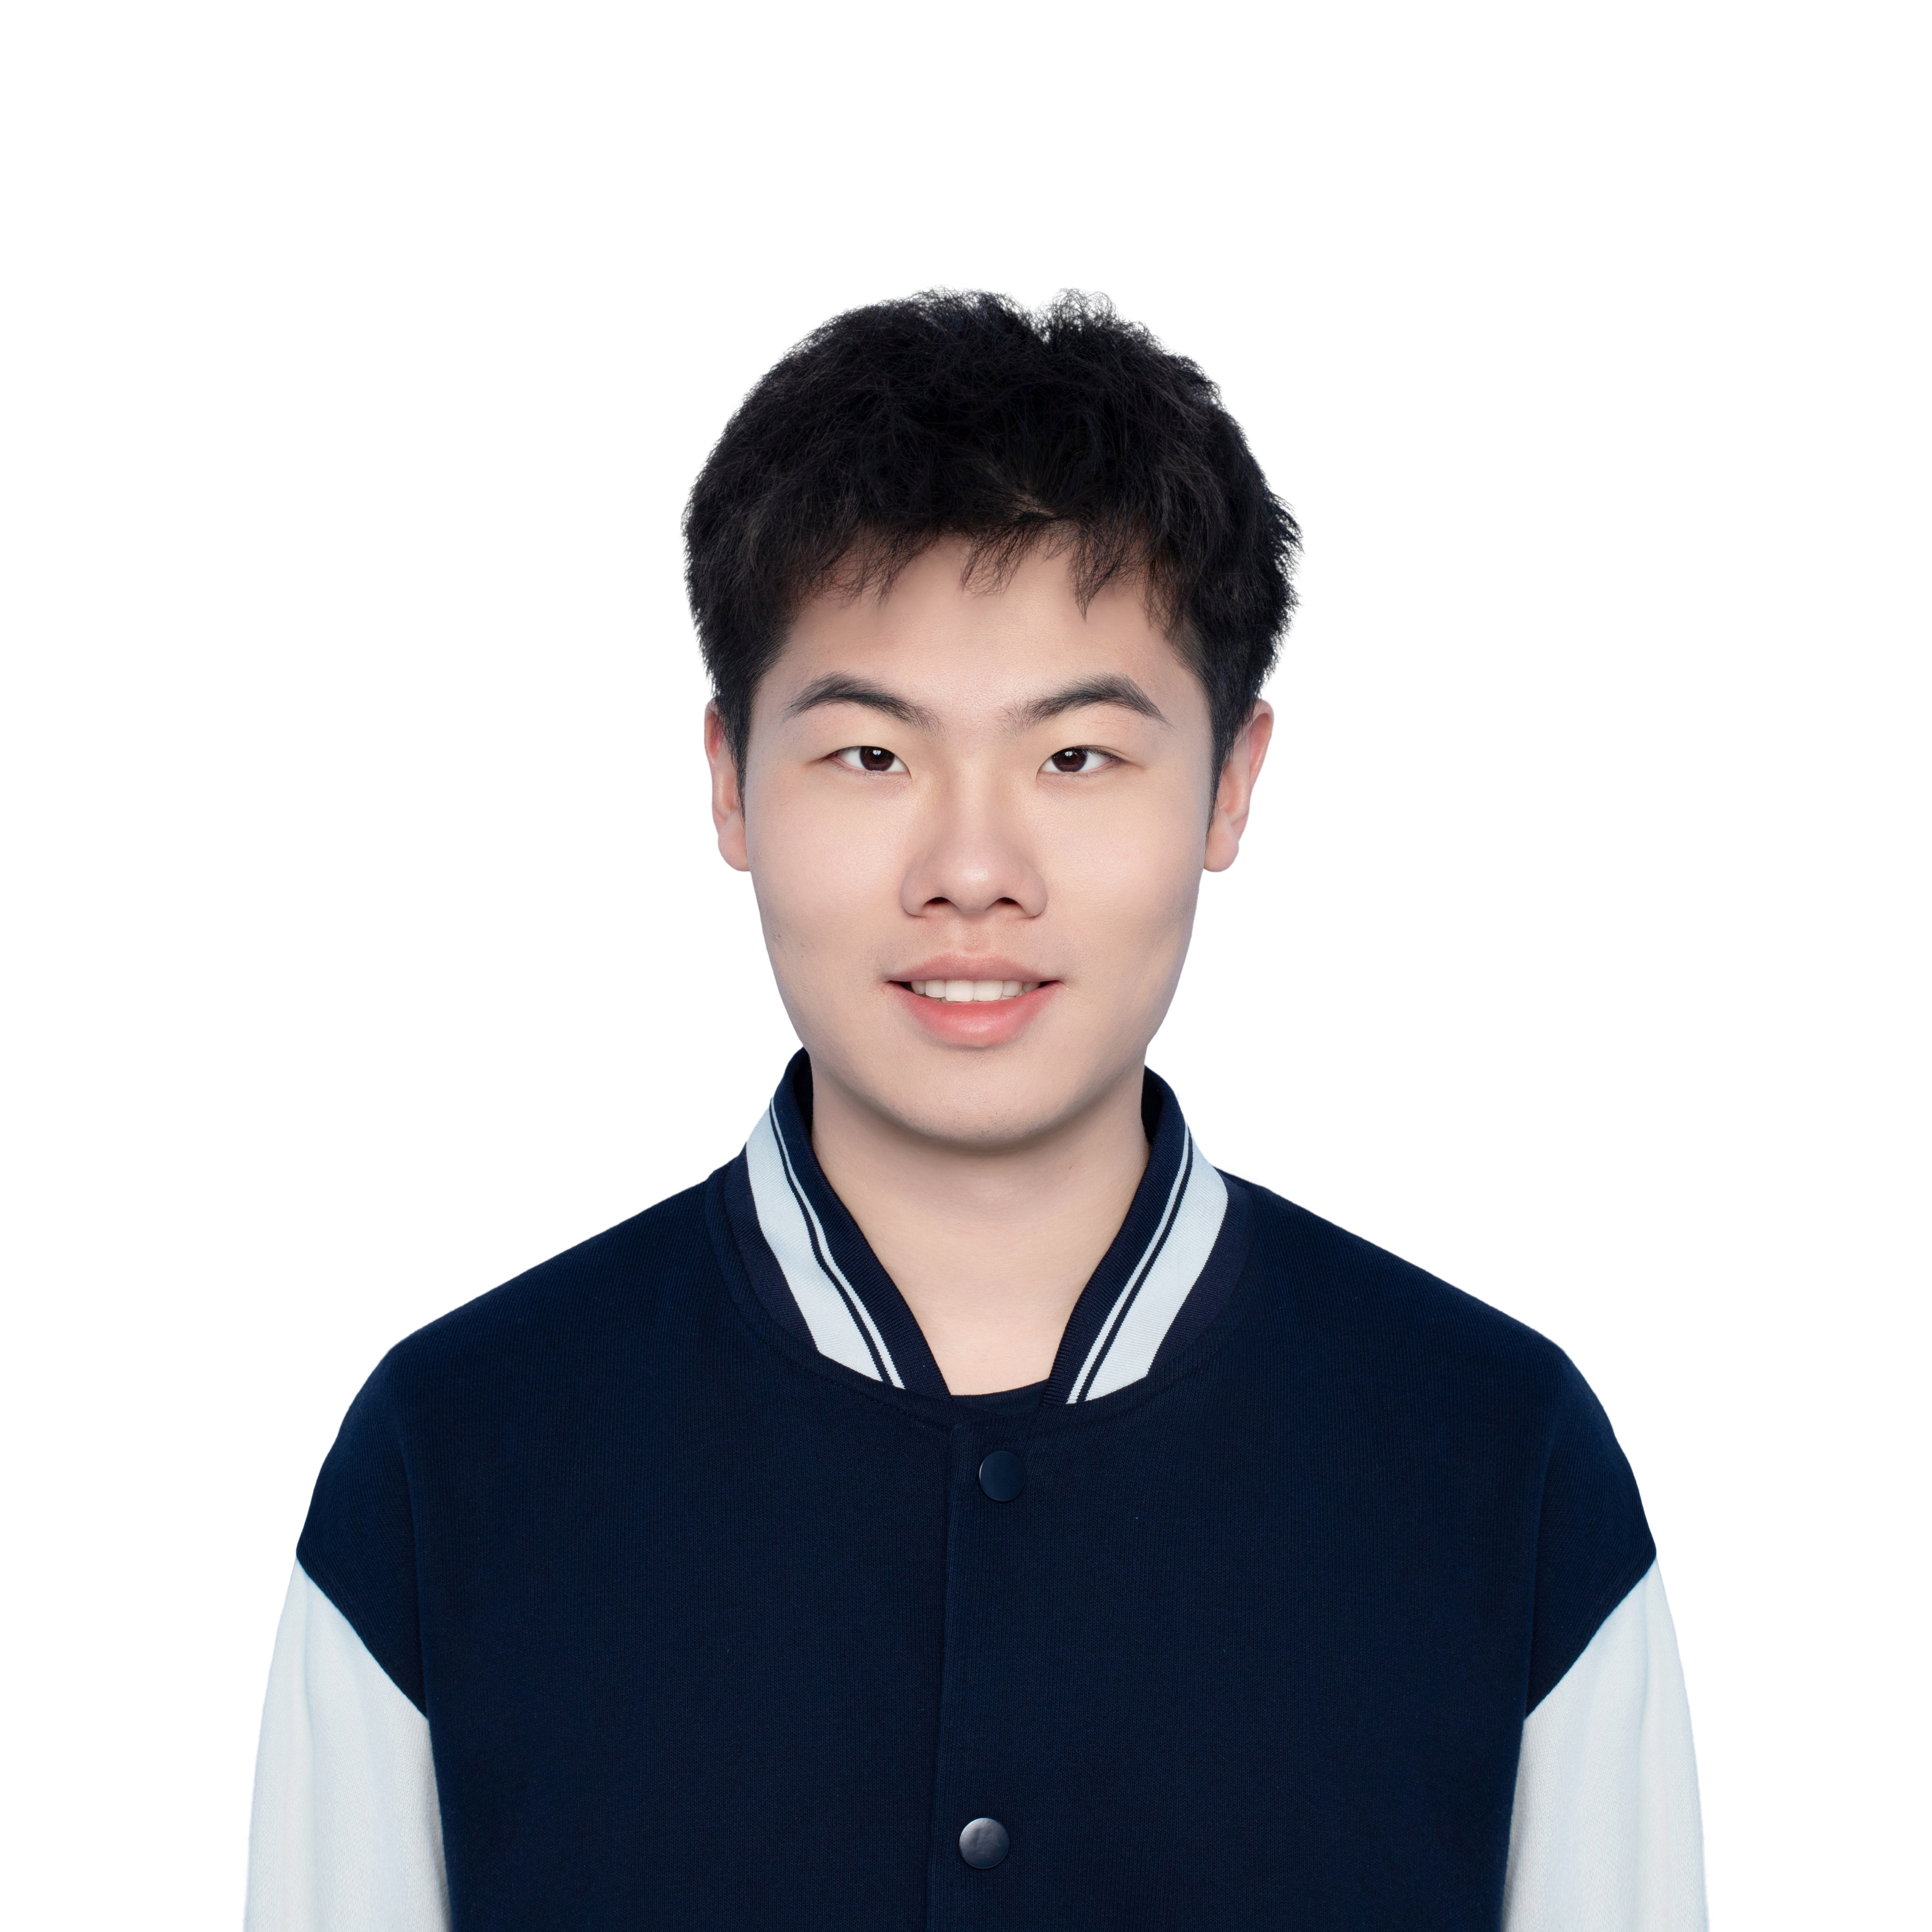
\includegraphics[height=2.5cm, keepaspectratio]{photo.JPG}};
\end{tikzpicture}%

\vspace{-2.4em}

% =====================================================================
% 双栏正文
% =====================================================================
\begingroup
\linespread{1.05}\selectfont
\begin{minipage}[t]{0.30\textwidth}
% 左栏偏窄：左对齐 + 禁连字断词，避免两端对齐在窄栏里拉出大间隙
\raggedright\hyphenpenalty=10000\exhyphenpenalty=10000\relax

% --- 教育 ---
\section{Education}
{\color{DescriptionGray}
\textbf{深圳北理莫斯科大学}\\[0.2em]
\begin{tabular*}{\linewidth}{@{}>{\raggedright\arraybackslash}b{0.66\linewidth}@{\extracolsep{\fill}}r@{}}
电子与计算机工程 学士 & 2024--2028\hspace*{0.5em}
\end{tabular*}
}

\vspace*{0.5em}
\subSection{校级荣誉}
{\color{DescriptionGray}
一等奖学金\\[0.2em]
优秀学生\\[0.2em]
科技创新优秀奖
}

% --- 方向 ---
\vspace*{\secgap}
\section{Interests}
{\color{DescriptionGray}
\textbf{算法与复杂性}\\[0.2em]
\textbf{学习理论与统计学}\\[0.2em]
\textbf{极值组合学}\par\vspace{0.35em}
\leftpara{我的工作横跨多个方向，始终关心的是一个问题的复杂度应当如何刻画，以及它最终由什么量决定。我享受把一个问题彻底闭环的过程，从证明下界、给出与之匹配的上界，到设计出达到这一界的算法。}
}

% --- 技能 ---
\vspace*{\secgap}
\section{Skills}
{\color{DescriptionGray}
\begin{tabular*}{\linewidth}{@{}l@{\extracolsep{\fill}}r@{}}
\skillRow{C++}{4}
\skillRow{Python}{3}
\skillRow{\LaTeX}{3}
\skillRow{MATLAB}{2}
\skillRow{Lean}{2}
\end{tabular*}}

% --- 语言 ---
\vspace*{\secgap}
\section{Languages}
{\color{DescriptionGray}
\begin{tabular*}{\linewidth}{@{}l@{\extracolsep{\fill}}r@{}}
Chinese & Native \\
English & Professional \\
Russian & Elementary \\
\end{tabular*}}

% --- 兴趣 ---
\vspace*{\secgap}
\section{Hobbies}
{\color{DescriptionGray}
\leftpara{钢琴、小提琴、架子鼓（中国音协 \mbox{10 级}优等）、羽毛球（校赛八强）、辩论（校赛亚军及最佳辩手）}
}

\end{minipage}%
\hfill
\begin{minipage}[t]{0.68\textwidth}

% --- 论文 ---
\section{Publications}
\begingroup
\hyphenpenalty=200\relax\exhyphenpenalty=200\relax\tolerance=1000\relax\emergencystretch=1em\relax\spaceskip=0.3333em plus 0.1667em minus 0.15em\relax

\textbf{Sichen Wang}.\ \href{https://sichenwang.com/publications/online-isotonic-regression/}{\textit{The Minimax Rate of Online Isotonic Regression on Product Orders}}.\ \href{https://openreview.net/forum?id=OZYmFCFi3w}{\textcolor{VenueColor}{NeurIPS 2026}}.
\par\vspace{\pubgap}
\textbf{Sichen Wang}, Zhipeng Lu.\ \href{https://sichenwang.com/publications/implicit-midpoint-langevin/}{\textit{Preconditioned Implicit Midpoint Langevin Sampling for Non-Smooth Bayesian Imaging}}.\ \href{https://openreview.net/forum?id=6vWdtoSoVB}{\textcolor{VenueColor}{NeurIPS 2026}}.
\par\vspace{\pubgap}
\textbf{Sichen Wang}, Zhipeng Lu.\ \href{https://sichenwang.com/publications/depth-over-fidelity/}{\textit{Depth over Fidelity in Fixed-Budget Noisy Evolution Strategies}}.\ \href{https://proceedings.mlr.press/v306/wang26ff.html}{\textcolor{VenueColor}{ICML 2026}}.

\endgroup

% --- Preprints ---
\vspace*{\secgap}
\section{Preprints}
\begingroup
\hyphenpenalty=200\relax\exhyphenpenalty=200\relax\tolerance=1000\relax\emergencystretch=1em\relax\spaceskip=0.3333em plus 0.1667em minus 0.15em\relax

\textbf{Sichen Wang}.\ \href{https://sichenwang.com/publications/denoising-flows-on-trees/}{\textit{The Minimax Rate of Denoising Flows on Trees}}.\ \href{https://arxiv.org/abs/2609.14091}{\textcolor{black}{arXiv:2609.14091}}.
\par\vspace{\pubgap}
\textbf{Sichen Wang}.\ \href{https://sichenwang.com/publications/unitary-synthesis-pspace-oracle/}{\textit{Unitary Synthesis with a PSPACE Oracle}}.
\par\vspace{\pubgap}
\textbf{Sichen Wang}.\ \href{https://sichenwang.com/publications/movement-complexity-of-sorting/}{\textit{The Movement Complexity of Sorting}}.\ \href{https://arxiv.org/abs/2611.01157}{\textcolor{black}{arXiv:2611.01157}}.
\par\vspace{\pubgap}
\textbf{Sichen Wang}, Zhipeng Lu, Jingbang Chen.\ \href{https://sichenwang.com/publications/price-of-order/}{\textit{The Price of Order in the Logarithmic Method}}.\ \href{https://arxiv.org/abs/2608.06388}{\textcolor{black}{arXiv:2608.06388}}.
\par\vspace{\pubgap}
\textbf{Sichen Wang}.\ \href{https://sichenwang.com/publications/tuza-conjecture/}{\textit{A Bound Below 2.8 for Tuza's Conjecture}}.\ \href{https://arxiv.org/abs/2609.13831}{\textcolor{black}{arXiv:2609.13831}}.

\endgroup

% --- 获奖 ---
\renewcommand{\arraystretch}{1.25}
\vspace*{\secgap}
\section{Awards}
\begin{tabular*}{\linewidth}{@{}l @{\extracolsep{\fill}} >{\raggedleft\arraybackslash}p{1.8cm}@{\hspace{-0.15em}} r@{}}
NOI 2022 冬令营 & \textbf{银牌} & \\
连续 3 年 CSP-S/NOIp & \textbf{一等奖} & \\
2024 ICPC 亚洲区域赛 (昆明, 沈阳) & \textbf{金牌} & Top 3\% \\
2024 CCPC 中国大学生程序设计竞赛 & \textbf{金牌} & Top 4\% \\
2024 ICPC 亚洲总决赛 (EC-Final) & \textbf{第 31 名} & Top 11\% \\
CCF CSP 计算机软件能力认证 & \textbf{480 分} & Top 0.1\% \\
\multicolumn{3}{@{}l@{}}{\makebox[\linewidth][l]{AdventureX 2025 黑客松\hfill\textbf{Vibe Coding 赛道冠军 / 中控算法赛道亚军}}} \\
\end{tabular*}

% --- 经历 ---
\vspace*{\secgap}
\section{Experience}

\subSection{Research}
\jobEntry{科研助理 @ 香港中文大学（深圳）}{Dec. 2024 -- Present}{与理工学院唐晓莹教授合作，研究大语言模型的基础问题}
\jobEntry{科研助理 @ 深圳北理莫斯科大学}{Nov. 2025 -- Present}{与工程系路志鹏老师合作，研究优化理论、极值组合与概率论}
\jobEntry{科研助理 @ 香港中文大学（深圳）}{Nov. 2025 -- Present}{与数据科学学院陈靖邦教授合作，研究算法分析、数据结构、图论与图挖掘}

\subSection{Industry}
\jobEntry{算法研究员 @ 增广智能}{May 2025 -- May 2026}{针对一类平面网格图上的数据调度问题提出「转向势能避让」方法，并撰写内部技术报告}

\subSection{Competitive Programming}
\jobEntry{讲师 @ NOI 2026 湖南省队集训}{Apr. 2026}{}
\jobEntry{讲师 @ 学军信友队暑期集训}{Jul. -- Aug. 2026}{}
\jobEntry{讲师 @ 中国计算机学会 · 信息学夏令营}{Aug. 2023}{}
\jobEntry{教练 @ 深北莫附中}{Aug. 2023 -- Feb. 2025}{受校长特聘，担任学校的信息学竞赛教练}
\jobEntry{出题人 @ 牛客竞赛}{}{独立完成 6 场比赛的命题与题解，每场参赛人数超过 2000}

\end{minipage}
\endgroup

\end{document}
